\documentclass{standalone}

%\usepackage{tgtermes}%
\usepackage{times}%
\usepackage[usenames,dvipsnames]{color}
\usepackage{tikz}
\usetikzlibrary{arrows,positioning,shadows}

\begin{document}

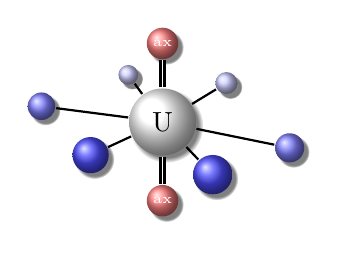
\begin{tikzpicture}
  [>=open triangle 45, thick,
  u/.style={ball color=black!0,
    circle,  circular drop shadow,
    inner sep=0pt,minimum size=8.5mm},
  o/.style={ball  color=blue!50,
    circle,  circular drop shadow,
    inner sep=0pt,minimum size=4mm},
  oback/.style={ball  color=blue!20,
    circle,  circular drop shadow,
    inner sep=0pt,minimum size=3mm},
  ofront/.style={ball  color=blue!70,
    circle, circular drop shadow, 
    inner sep=0pt,minimum size=5mm},
  oax/.style={ball  color=red!50,
    circle, circular drop shadow,
    inner sep=0pt,minimum size=4mm},
  c/.style={ball  color=black,
    circle, 
    inner sep=0pt,minimum size=6mm},
  p/.style={ball  color=black,
    circle, 
    inner sep=0pt,minimum size=7mm},
  ueqbond/.style={solid},
  dbond/.style={thick, double, solid},
  null/.style={shape=circle, fill=white,
    inner sep=0pt,minimum size=1mm},
  ]  % circular drop shadow,

  \begin{scope}[yshift=-180,yslant=0.5,xslant=-1]
    \node[u] (U) at (0,0,0) {U};

    %% bottom axial oxygen + double bond
    \node[oax] (Oax2) at (-1.01652*1.6,-1.01652*1.6,-1.01652*1.6)
    [white] {\tiny ax};
    \draw[dbond] (U) to (Oax2);


    \node[oback,minimum size=2.5mm] (Oeq3) at ( 0.76213/4, 1.25061/2,-1.97853/4) {}; %3
    \node[ofront] (Oeq4) at (-0.49169/3,-1.44195/1.8, 1.94112/4) {}; %4
    \node[oback,minimum size=2.8mm] (Oeq6) at ( 1.94112/3,-0.49169/3,-1.44195/2.2) {}; %6

    %% carbonyl/carbonate
    \node[ofront,minimum size=4.6mm] (Oeq2) at (-1.97853/3, 0.76213/3, 1.25061/2.2) {}; %2
    \node[o,minimum size=3.5mm] (Oeq5) at (-1.44195/2.2, 1.94112/2.2,-0.49169/2.2) {}; %5
    % \node[c] (C1) at (-2.17414/1.4, 1.77010/1.4, 0.52590/1.4) [white] {C};
    % \node[c] (C2) at (-2.17414, 1.77010, 0.52590) [white] {C};
%    0.52590   -2.17414    1.77010  4  C.1           2.85249
%    1.77010    0.52590   -2.17414  4  C.1           2.85249

    % \draw[solid] (C1) to (Oeq5);
    % \draw[solid] (C1) to (Oeq2);
    % \draw[dbond] (C1) to (C2);

    %% phosphoryl
    \node[o,minimum size=3.7mm] (Oeq1) at ( 1.25061/2,-1.97853/2, 0.76213/2) {}; %1
    % \node[p] (P) at ( 1.25061*0.8,-1.97853*0.8, 0.76213*0.8) [white] {P};
    % \draw[solid] (Oeq1) to (P);

    % \node[o] (OP1) at ( 1.25061*1.1+0.7,-1.97853*1.1+1, 0.76213*1.1+0.6) [white] {};
    % \node[o] (OP2) at ( 1.25061*1.1-0.9,-1.97853*1.1-0.2, 0.76213*1.1+0.) [white] {};
    % \node[o] (OP3) at ( 1.25061*1.1-0.4,-1.97853*1.1-0.2, 0.76213*1.1-0.6) [white] {};

    % \draw[solid] (P) to (OP1);
    % \draw[solid] (P) to (OP2);
    % \draw[solid] (P) to (OP3);



    \draw[ueqbond] (U) to (Oeq1);
    \draw[ueqbond] (U) to (Oeq2);
    \draw[ueqbond] (U) to (Oeq3);
    \draw[ueqbond] (U) to (Oeq4);
    \draw[ueqbond] (U) to (Oeq5);
    \draw[ueqbond] (U) to (Oeq6);
    
    %% top axial oxygen + double bond
    \node[oax] (Oax1) at ( 1.01332*1.6, 1.01332*1.6, 1.01332*1.6)
    [white] {\tiny ax};
    \draw[dbond] (U) to (Oax1);

    \node[null] (nu) at ( +0.15, -1.7, 1.3) {};
  \end{scope}
  

\end{tikzpicture}

\end{document}


%%% Local Variables:
%%% mode: latex
%%% TeX-master: t
%%% TeX-parse-self: t
%%% TeX-auto-save: t
%%% TeX-auto-untabify: t
%%% TeX-PDF-mode: t
%%% eval: (flyspell-mode 1)
%%% End:
